\FChapter{Chapter Thirty-Eight}{38}

\Lettrine{R}{eader,} \textsc{I married him.} A quiet wedding we had: he and I, the parson and
clerk, were alone present. When we got back from church, I went into
the kitchen of the manor-house, where Mary was cooking the dinner and
John cleaning the knives, and I said---

\enquote{Mary, I have been married to \Mr{} Rochester this morning.} The
housekeeper and her husband were both of that decent phlegmatic order of
people, to whom one may at any time safely communicate a remarkable
piece of news without incurring the danger of having one's ears pierced
by some shrill ejaculation, and subsequently stunned by a torrent of
wordy wonderment. Mary did look up, and she did stare at me: the ladle
with which she was basting a pair of chickens roasting at the fire, did
for some three minutes hang suspended in air; and for the same space of
time John's knives also had rest from the polishing process: but Mary,
bending again over the roast, said only---

\enquote{Have you, Miss? Well, for sure!}

A short time after she pursued---\enquote{I seed you go out with the
master, but I didn't know you were gone to church to be wed;} and she
basted away. John, when I turned to him, was grinning from ear to ear.

\enquote{I telled Mary how it would be,} he said: \enquote{I knew what
\Mr{} Edward} (John was an old servant, and had known his master when he
was the cadet of the house, therefore, he often gave him his Christian
name)---\enquote{I knew what \Mr{} Edward would do; and I was certain he
would not wait long neither: and he's done right, for aught I know. I
wish you joy, Miss!} and he politely pulled his forelock.

\enquote{Thank you, John. \Mr{} Rochester told me to give you and Mary
this.} I put into his hand a five-pound note. Without waiting to hear
more, I left the kitchen. In passing the door of that sanctum some time
after, I caught the words---

\enquote{She'll happen do better for him nor ony o't' grand ladies.} 
And again, \enquote{If she ben't one o' th' handsomest, she's noan faâl
and varry good-natured; and i' his een she's fair beautiful, onybody may
see that.}

I wrote to Moor House and to Cambridge immediately, to say what I had
done: fully explaining also why I had thus acted. Diana and Mary
approved the step unreservedly. Diana announced that she would just
give me time to get over the honeymoon, and then she would come and see
me.

\enquote{She had better not wait till then, Jane,} said \Mr{} Rochester,
when I read her letter to him; \enquote{if she does, she will be too
late, for our honeymoon will shine our life long: its beams will only
fade over your grave or mine.}

How \St{} John received the news, I don't know: he never answered the
letter in which I communicated it: yet six months after he wrote to me,
without, however, mentioning \Mr{} Rochester's name or alluding to my
marriage. His letter was then calm, and, though very serious, kind. He
has maintained a regular, though not frequent, correspondence ever
since: he hopes I am happy, and trusts I am not of those who live
without God in the world, and only mind earthly things.

You have not quite forgotten little Adèle, have you, reader? I had not;
I soon asked and obtained leave of \Mr{} Rochester, to go and see her at
the school where he had placed her. Her frantic joy at beholding me
again moved me much. She looked pale and thin: she said she was not
happy. I found the rules of the establishment were too strict, its
course of study too severe for a child of her age: I took her home with
me. I meant to become her governess once more, but I soon found this
impracticable; my time and cares were now required by another---my
husband needed them all. So I sought out a school conducted on a more
indulgent system, and near enough to permit of my visiting her often,
and bringing her home sometimes. I took care she should never want for
anything that could contribute to her comfort: she soon settled in her
new abode, became very happy there, and made fair progress in her
studies. As she grew up, a sound English education corrected in a great
measure her French defects; and when she left school, I found in her a
pleasing and obliging companion: docile, good-tempered, and
well-principled. By her grateful attention to me and mine, she has long
since well repaid any little kindness I ever had it in my power to offer
her.

My tale draws to its close: one word respecting my experience of married
life, and one brief glance at the fortunes of those whose names have
most frequently recurred in this narrative, and I have done.

I have now been married ten years. I know what it is to live entirely
for and with what I love best on earth. I hold myself supremely
blest---blest beyond what language can express; because I am my
husband's life as fully as he is mine. No woman was ever nearer to her
mate than I am: ever more absolutely bone of his bone and flesh of his
flesh. I know no weariness of my Edward's society: he knows none of
mine, any more than we each do of the pulsation of the heart that beats
in our separate bosoms; consequently, we are ever together. To be
together is for us to be at once as free as in solitude, as gay as in
company. We talk, I believe, all day long: to talk to each other is but
a more animated and an audible thinking. All my confidence is bestowed
on him, all his confidence is devoted to me; we are precisely suited in
character---perfect concord is the result.

\Mr{} Rochester continued blind the first two years of our union; perhaps
it was that circumstance that drew us so very near---that knit us so
very close: for I was then his vision, as I am still his right hand. 
Literally, I was (what he often called me) the apple of his eye. He saw
nature---he saw books through me; and never did I weary of gazing for
his behalf, and of putting into words the effect of field, tree, town,
river, cloud, sunbeam---of the landscape before us; of the weather round
us---and impressing by sound on his ear what light could no longer stamp
on his eye. Never did I weary of reading to him; never did I weary of
conducting him where he wished to go: of doing for him what he wished to
be done. And there was a pleasure in my services, most full, most
exquisite, even though sad---because he claimed these services without
painful shame or damping humiliation. He loved me so truly, that he
knew no reluctance in profiting by my attendance: he felt I loved him so
fondly, that to yield that attendance was to indulge my sweetest wishes.

One morning at the end of the two years, as I was writing a letter to
his dictation, he came and bent over me, and said---\enquote{Jane, have
you a glittering ornament round your neck?}

I had a gold watch-chain: I answered \enquote{Yes.}

\enquote{And have you a pale blue dress on?}

\begin{figure}
	\begin{sidecaption}{\enquote{And have you a pale blue\linebreak dress on?}}[p435b]
		\centering
		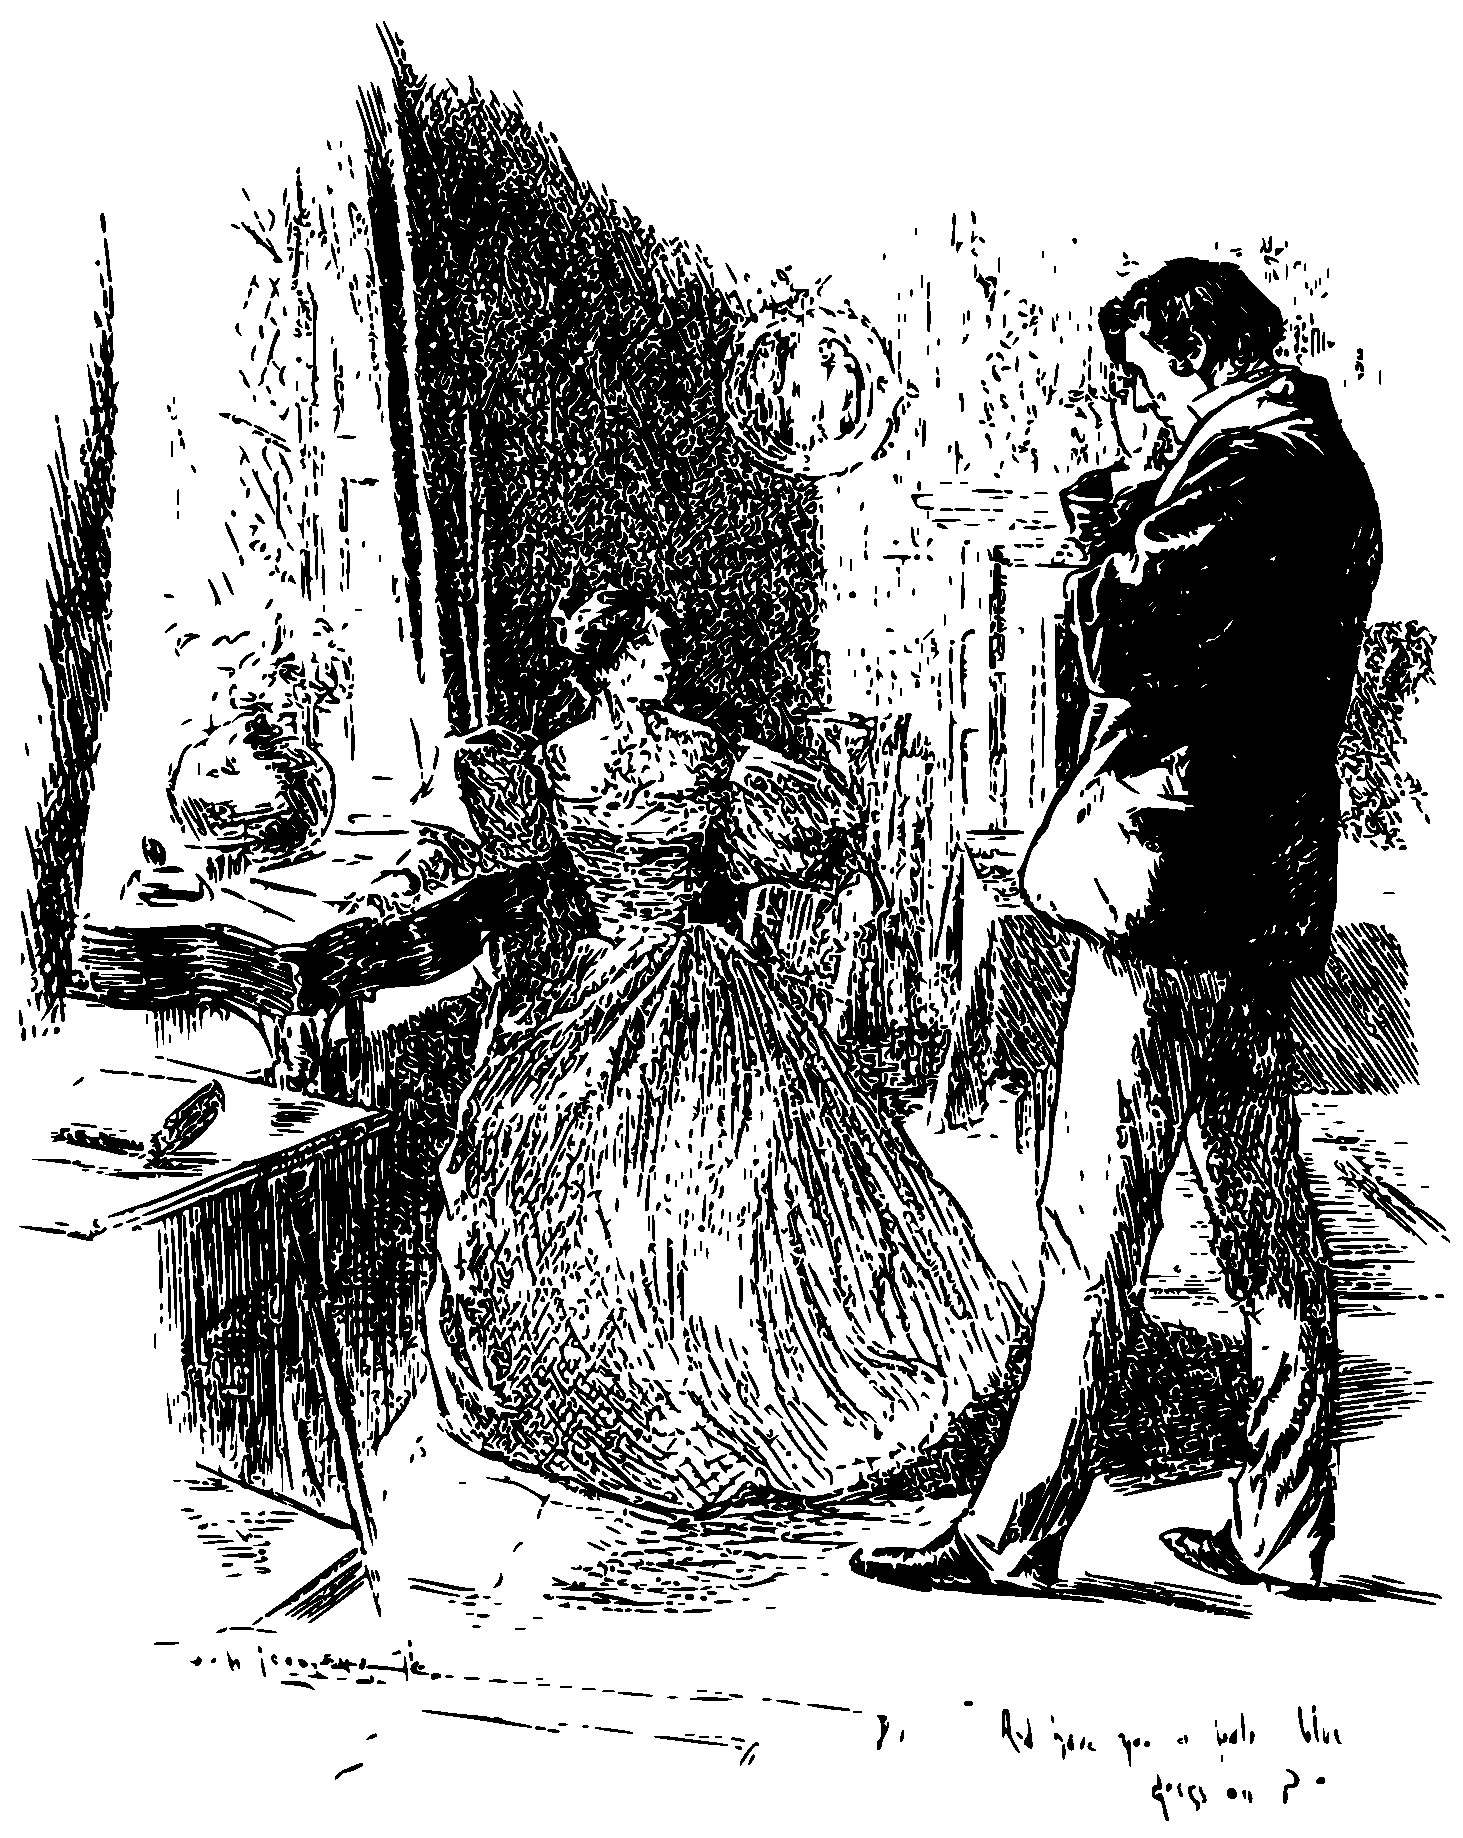
\includegraphics[width=\linewidth]{images/p435b.pdf}
	\end{sidecaption}
\end{figure}

I had. He informed me then, that for some time he had fancied the
obscurity clouding one eye was becoming less dense; and that now he was
sure of it.

He and I went up to London. He had the advice of an eminent oculist;
and he eventually recovered the sight of that one eye. He cannot now
see very distinctly: he cannot read or write much; but he can find his
way without being led by the hand: the sky is no longer a blank to
him---the earth no longer a void. When his first-born was put into his
arms, he could see that the boy had inherited his own eyes, as they once
were---large, brilliant, and black. On that occasion, he again, with a
full heart, acknowledged that God had tempered judgment with mercy.

My Edward and I, then, are happy: and the more so, because those we most
love are happy likewise. Diana and Mary Rivers are both married:
alternately, once every year, they come to see us, and we go to see
them. Diana's husband is a captain in the navy, a gallant officer and a
good man. Mary's is a clergyman, a college friend of her brother's,
and, from his attainments and principles, worthy of the connection. 
Both Captain Fitzjames and \Mr{} Wharton love their wives, and are loved
by them.

As to \St{} John Rivers, he left England: he went to India. He entered on
the path he had marked for himself; he pursues it still. A more
resolute, indefatigable pioneer never wrought amidst rocks and dangers. 
Firm, faithful, and devoted, full of energy, and zeal, and truth, he
labours for his race; he clears their painful way to improvement; he
hews down like a giant the prejudices of creed and caste that encumber
it. He may be stern; he may be exacting; he may be ambitious yet; but
his is the sternness of the warrior Greatheart, who guards his pilgrim
convoy from the onslaught of Apollyon. His is the exaction of the
apostle, who speaks but for Christ, when he says---\enquote{Whosoever
will come after me, let him deny himself, and take up his cross and
follow me.} His is the ambition of the high master-spirit, which aims
to fill a place in the first rank of those who are redeemed from the
earth---who stand without fault before the throne of God, who share the
last mighty victories of the Lamb, who are called, and chosen, and
faithful.

\St{} John is unmarried: he never will marry now. Himself has hitherto
sufficed to the toil, and the toil draws near its close: his glorious
sun hastens to its setting. The last letter I received from him drew
from my eyes human tears, and yet filled my heart with divine joy: he
anticipated his sure reward, his incorruptible crown. I know that a
stranger's hand will write to me next, to say that the good and faithful
servant has been called at length into the joy of his Lord. And why
weep for this? No fear of death will darken \St{} John's last hour: his
mind will be unclouded, his heart will be undaunted, his hope will be
sure, his faith steadfast. His own words are a pledge of this---

\enquote{My Master,} he says, \enquote{has forewarned me. Daily He
announces more distinctly,---\enquote{Surely I come quickly!} and hourly I more
eagerly respond,---\enquote{Amen; even so come, Lord Jesus!}}
